%%%%%%%%%%%%%%%%%%%%%%%%%%%%%%%%%%%%%%%%%%%%%%%%%%%%%%%%%%%%%%%%%%%%%%%%%%%%%%%%%%%%%%%%%
% SECTION HYDRODYNAMIC SIMULATIONS 
%%%%%%%%%%%%%%%%%%%%%%%%%%%%%%%%%%%%%%%%%%%%%%%%%%%%%%%%%%%%%%%%%%%%%%%%%%%%%%%%%%%%%%%%%

\chapter{Hydrodynamic Simulations}
\section{2D Simulations}
\new{
	The physics of 2D hydrodynamic is qualitatively very similar but quantitatively very different to the 3D case. Concepts such as hydrostatic equilibrium or the Schwarzschild criterion can be applied in 2D as well as in 3D, but the resulting flows will have different properties. Turbulence for instance in the 2D case transfers kinetic energy from small eddies to large eddies, while in the 3D case the opposite happens. We expect hence the entrainment mass ratio to be different between the 2D and 3D cases. 
	
	Nevertheless, being 2D simulations computationally so cheap, they are a very useful tool to make experience with the code and to run tests in order to setup bigger and more expensive 3D runs. In our case for instance it was necessary to have a rough estimate of the entrainment rate, of the boundary migration velocity and of the convective turnover timescale.

	
}
\subsection{Simulations setup}
The physical setup used for our simulations is the so called "box in a star" method, meaning that we simulate some relatively very small internal region of a star. 

In our case for the 2D runs it will be a box of $2.50 \times 10^{9} \ \mathrm{cm}$ on the $x$ axis and $1.25 \times 10^{9} \ \mathrm{cm}$ on the $y$ axis. Gravity is constantly pointing downward on the $y$ axis with a magnitude of $1000 \mathrm{cm/s^2}$. This generates a pressure stratification in the fluid that covers approximately three pressure scale heights. 

The controlling parameter in our setup is the temperature gradient that can be initialized to any value. In our case we divided the simulated region in three parts. The bottom region (labeled as $1$) starts at the lower boundary and reaches $4/12$ of the domain, the central (labeled as $2$) proceeds until the middle, and the upper one (labeled as $3$) reaches the upper boundary, as shown in \ref{fig:tempprofile}. We define a parameter $\alpha_{i}$ ($i=1, 2, 3$) which is nothing but the fraction of the $\nabla$ over the $\nabla_{\mathrm{ad}}$. As seen in previous sections $\alpha_{i}<1$ implies stability in the $i-$region, instability otherwise. 

We always initialized the setup with $\alpha_{1} = \alpha_{3}$ widely smaller than $1$; and $\alpha_{2}=0.99$, which means a very precarious situation in terms of stability in the second region. 

A heating function furthermore heats the second region with a Gaussian profile (see figure \ref{fig:twin}) to stimulate convection. Without it the system would never become convective in the first place, since hydrostatic equilibrium is fulfilled everywhere. Furthermore the heating function keeps the system convectively unstable. In fact without the constant energy generation because of heat mixing and numerical viscosity, the system would soon reach again a stable configuration of hydrostatic equilibrium. This mimics the energy generations in deep stellar interiors provided by nuclear burning. The choice of a Gaussian profile is a common praxis in stellar physics. On the one hand we require that the heating is peaked deep inside the convective region and that it does not influences the stable layers, on the other hand it is preferable not to use functions with discontinuity, because this might generate shock waves that propagate into the system.

The values of $\alpha_{1}$ and $\alpha_{3}$ are controlling parameters for the bulk-Richardson number, since they are proportional to $\Delta b$. The advantage of simulating a strip of convection between two stable layers (miming a Shell convection) instead of a convective region at the bottom that grows upward (core convection-like) is twofold: it gives us two convective boundaries to study instead of one, and we avoid high Mach number at the boundary which can at times generate problems or unphysical situations. 

One of the hardest tasks has been to generate the correct amount of heating such that the turbulence standard deviation \textit{at the interface} was constant during the run (which is one of the ingredients of the bulk-Richardson number, hence one of the parameters we want to control in order to perform a differential study). In order to do that, the heating function is tuned such that, at $t=100K \ \mathrm{s}$ the total heat generation is reduced to $50 \%$ of the original amount.

\begin{figure}[t]
\centering
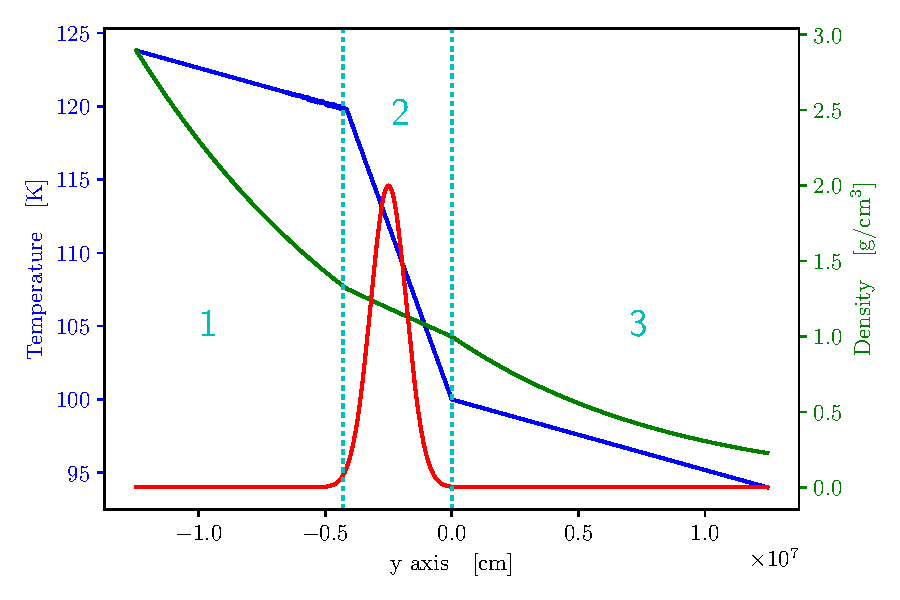
\includegraphics[width=10cm]{./img/twin.pdf}
\caption{Example of initial temperature (blue) and pressure (red) profile along the $y$-axis. The red curve represents the shape of the heating function in arbitrary unit.}
\label{fig:twin}
\centering
\end{figure}
At the bottom of the simulated region small perturbations in temperature and Mach number had been imprinted on the stratification in order to break the initial symmetry of the system.

A wide range of boundary conditions have been tested for this problem. In our first setup we used to stimulate convection at the bottom of the simulated region, but implementing periodic boundaries (that definitely provide the most physical situation) a shear flow appeared in both the stable and convective region at the onset of convection. We then tested reflective boundaries and wall boundaries. In the first case we observed a mass loss (very likely because of a bug in the code). In the second case after a few tens of minutes of the onset of convection, a spike in the Mach number at the boundary appeared, and the code crashed. Interestingly enough, the spike appeared always at the left boundary. For this reason we initially suspected another bug in the code. What actually used to happen is that some fluid stagnated right above the convective boundary (specifically the first column of cell on the left) and over time a massive temperature gradient was established. We suppose that this computational artifact appeared only on one side of the grid because the iterative linear solvers implemented in SLH are not perfectly symmetric. This is generally not a source of problems unless in specific pathologic cases as the one we had to face. We then tested a new setup, where convection was stimulated in the central region of the domain. By implementing periodic boundaries the same shear flow appeared, but only after a few tens of hours of simulated time, which allowed us to collect enough data for the analysis. For the vertical direction we used wall boundary conditions. As we will explain this is not a perfectly physical solution, since internal modes can bounce on them and be reflected.

As briefly explained in the previous sections, in order to define the topology of the convective boundaries, we initialized a passive scalar inside each one of the regions. Recall that passive scalars are just like colors of the fluid and in no way influence the dynamics of the system, nor do they diffuse.

As previously stated our goal is to perform a \textit{differential} study of the bulk-Richardson number and the CBM problem. This implies running simulations with different values of $\Delta b$ and $\sigma_t$ at different resolutions. Being that 2D simulations computationally so cheap, we managed to run a copious amount of them. With the code 2d0.10-0.80 we will refer to a 2-dimensional run with $\alpha_{1} = \alpha_{3}=0.1$ and $80 \%$ of the heating referring to the arbitrary value of $4.5 10^{15} \mathrm{erg/s}$.

We run in 2D on a $2048 \times 1024$ uniform Cartesian grid. It is worth remarking that when doing CFD with a higher resolution, one not only better resolves the features of the system, but also decreases the numerical viscosity (increases the Reynolds number). This is the reason for which we chose this grid setup: we want to keep cells squared and keep viscosity a scalar quantity, and prevent it from becoming a tensorial one. In the next section we will perform a convergence study, in order to understand which roles the resolution and the viscosity play in the phenomenon of convective entrainment.


\subsection{Evolution of a single run}
\begin{figure}[t!]
      \centering
      \subfloat[Mach number profile over time.]{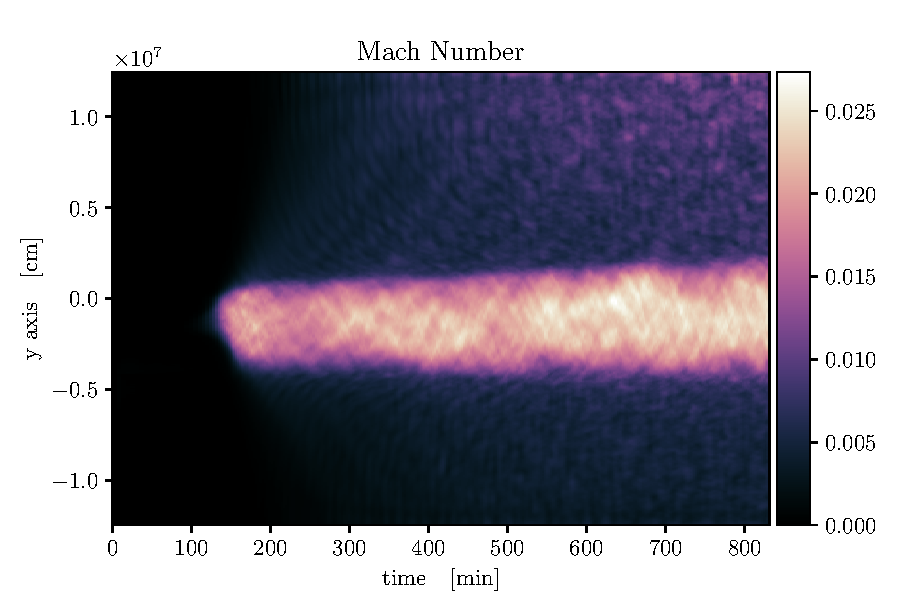
\includegraphics[width=12cm]{./img/mach.pdf}\label{fig:2dmachprofile}}
     \centering
	\hfill
	\subfloat[Entrainment of the third passive scalar from the upper stable region (region 3) in the convective region.]{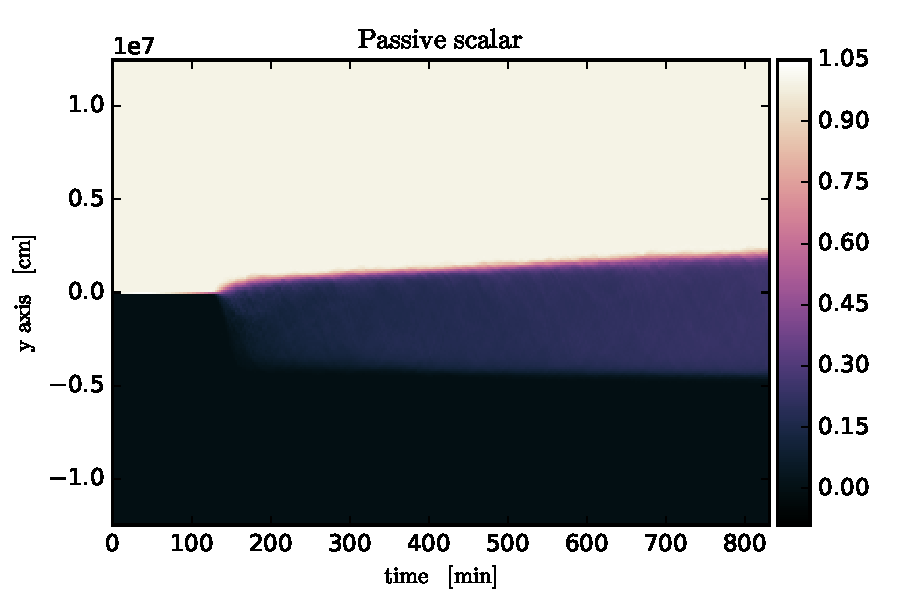
\includegraphics[width=12cm]{./img/ps2.pdf}\label{fig:2dpsprofile}}
	\caption{Time evolution of a 2D run for the Mach number and the third passive scalar (average on the horizontal direction).}
	\label{fig:2dsinglefirst}
\end{figure}
Let's consider the setup 2d0.10-0.80. 

Convection starts at around $t \sim 150 \mathrm{min}$. Because of the already mentioned implicit time stepping, the lower the Mach number, the bigger the time step, allowing us to save a huge amount of computational resources before the rise of convection. A remarkable difference is also observed in the convective regime, as long as the Mach number is below $10 \%$, which has always been our case.

\begin{figure}[t!]
  \centering
  \subfloat[Advection of the second passive scalar in the central region (region 2) at the onset of convective motions, at $t \simeq 150 \ \mathrm{min}$]{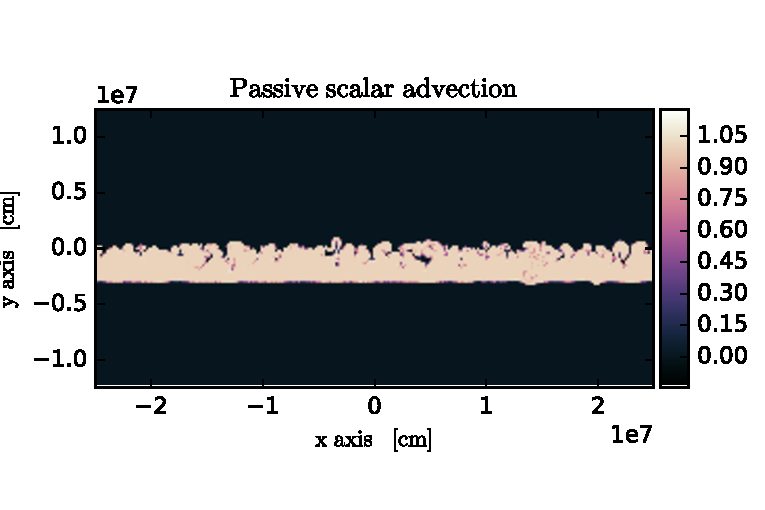
\includegraphics[width=12cm]{./img/passiveacc1.pdf}\label{fig:passiveacc1}}
  \centering
  \hfill
  \subfloat[The same passive scalar of above, advected at $t \simeq 800 \ \mathrm{min}$. This defines the topology of the boundary.]{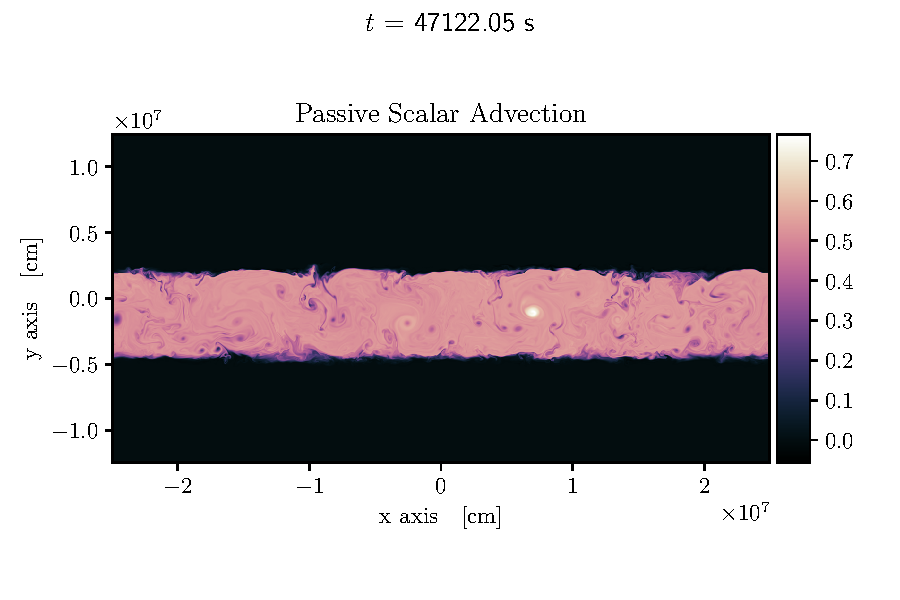
\includegraphics[width=12cm]{./img/passiveacc2.pdf}\label{fig:passiveacc2}}
  \caption{\new{Advection of the passive scalar initialized in the central region over the simulated time}}
  \end{figure}
In figure \ref{fig:2dmachprofile} we plot the profile of the Mach number over the simulated time. Convection starts at around $t=150 \mathrm{min}$ in the central region (region 2), while the upper and lower region remain stable. Some time is needed for convection so start, because the fluid needs to be heated to an unstable configuration. One can also observe that the convective region expands over time, i.\ e.\ the upper boundary moves upward and the lower boundary downward. Two remarks that need to be done. 

First of all the Mach number is stable over time, thanks to the heating function that we implemented, featuring a decrease of heat generation as previously explained. 
Second it is clear that some internal modes are excited by the convective blobs when they hit the stable layers and they propagate through them. They appear more significant in the upper region and to a certain extent this is true, but mainly this is due to the fact that the speed of sound there is lower. The difference is not so dramatic when plotting the absolute velocity. Two interesting questions remain without answer. First of all it is impossible to tell to which extent the dynamic of the boundary is influenced by these modes. Second of all it is possible that the chemical mixing due to these modes in the stable stratification might have a significant impact on the evolution of a star, which is obviously not considered in 1-D simulations. We believe that further investigations of this hypothesis are needed.

  In figure \ref{fig:2dpsprofile} we plot the third passive scalar (initialized in the upper region), which over time is entrained by convection. We clearly see the movement of the boundaries that over the $800 \ \mathrm{min}$ of simulated time move gradually upward and downward. As previously mentioned the first passive scalar was initialized in the lower region (region 1), and consequently advected into the convective region. A Lagrangian study of entrainment consists in quantifying the amount of passive scalar ingested at each boundary over time, i.\ e.\ integrating each passive scalar density over the convective region at every time step, and analyze the growth of this quantity over time.

\begin{figure}[t!]
\centering
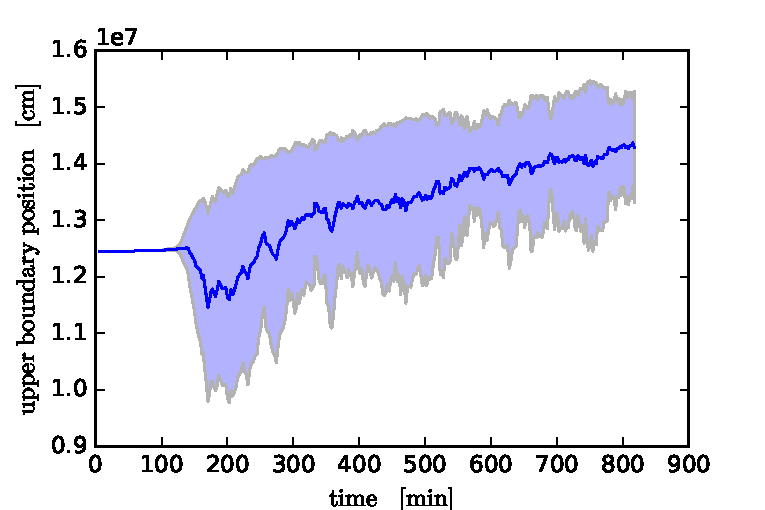
\includegraphics[width=0.6\textwidth]{./img/boundpos.pdf}
\caption{Boundaries positions over time. Shaded regions represent the boundary thickness (see text). Blue lines represent the upper boundary, green lines the lower boundary.}
\label{fig:boundpos}
\end{figure}
  As previously mentioned a second passive scalar was initialized in the central region (region 2). The use of this was not for an entrainment study, but to define the boundary position and its topology. In Figure (\ref{fig:passiveacc1}) we show the central passive scalar at the onset of convection. The growth of the first convective blobs is clearly visible. In the next $650 \mathrm{min}$ this dye will be advected everywhere in the convective region as it can be clearly seen in Figure (\ref{fig:passiveacc2}). We define the boundary position as the surface where the gradient of the concentration of the second passive scalar decreases the most. This holds for both the upper and lower boundary.
  
  For the runs with lower resolution this method worked perfectly but when moving to a higher resolution, a problem appeared. As the red arrow in Figure (\ref{fig:passiveacc2}) shows, in the middle of the convective layer some blobs of entrained material appear, that even when fully in a convective regime, still do not contain any passive scalar. This is due to the fact that the higher the resolution, the lower the numerical diffusion.
  
  This obviously is a problem for the boundary definition, because when looking for the highest drop in passive scalar concentration, one finds a value that has nothing to do with the boundary position. If we take as an example Figure (\ref{fig:passiveacc2}) for instance, the position detected by our script for the upper and lower boundary at $x \simeq -1 \times 10^{7} \mathrm{cm}$ is at around $y \simeq 0 \mathrm{cm}$. This could make sense for the upper boundary, but definitely not for the lower boundary, since its initial position is at $y=-0.4 \times 10^{7} \mathrm{cm}$ and we expect it to moves downward. We fixed this problem in out analysis script by checking if the automatically detected boundary position was before the initial position. If this was the case the script automatically considers the data corrupted, and substitute it with the mean value of the other positions. For the future simulations that we are planning to run, we are considering to constantly inject over time some passive scalar deep in the convective region, to make sure that after half a convective turnover at the most, all the convective medium has a non-zero concentration of passive scalar.

\begin{figure}[t!]
  \centering
    \subfloat[Buoyancy jump over time.]{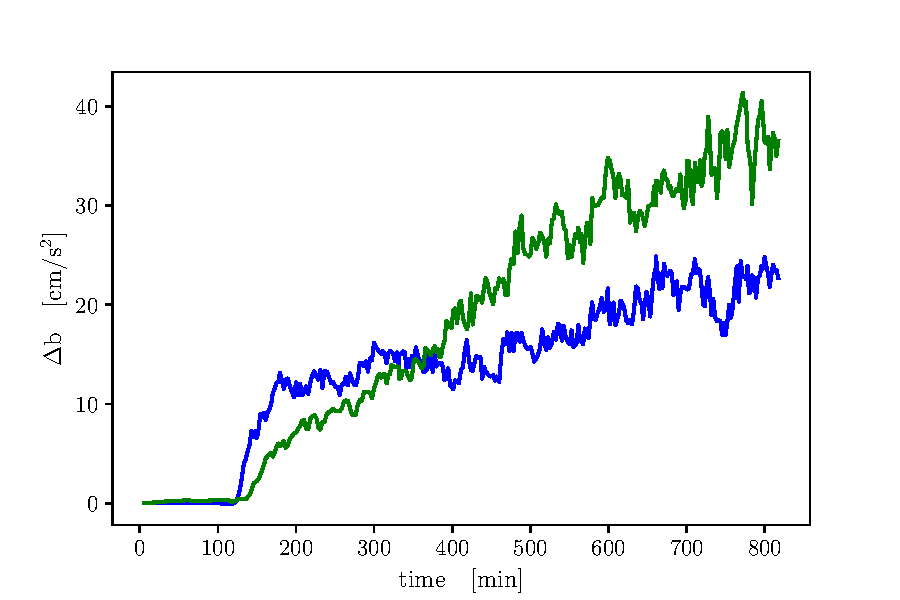
\includegraphics[width=0.5\textwidth]{./img/delb.pdf}\label{fig:delb}}
      \hfill
        \subfloat[Turbulence length scale over time.]{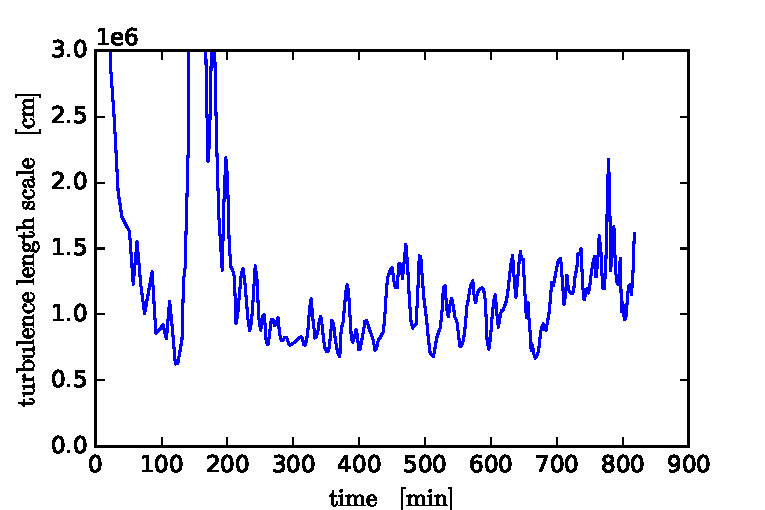
\includegraphics[width=0.5\textwidth]{./img/len.pdf}\label{fig:len}}
	\hfill
  \centering
    \subfloat[Turbulence standard deviation over time.]{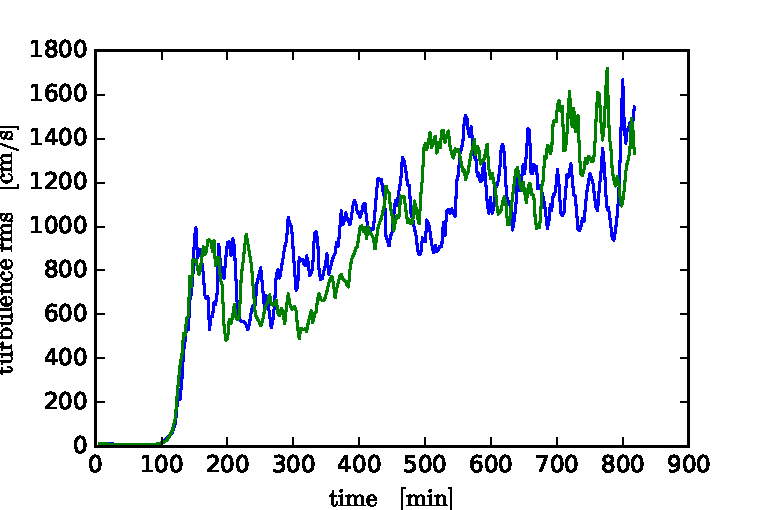
\includegraphics[width=0.5\textwidth]{./img/sigt.pdf}\label{fig:sigt}}
      \hfill
        \subfloat[Entrained mass over time.]{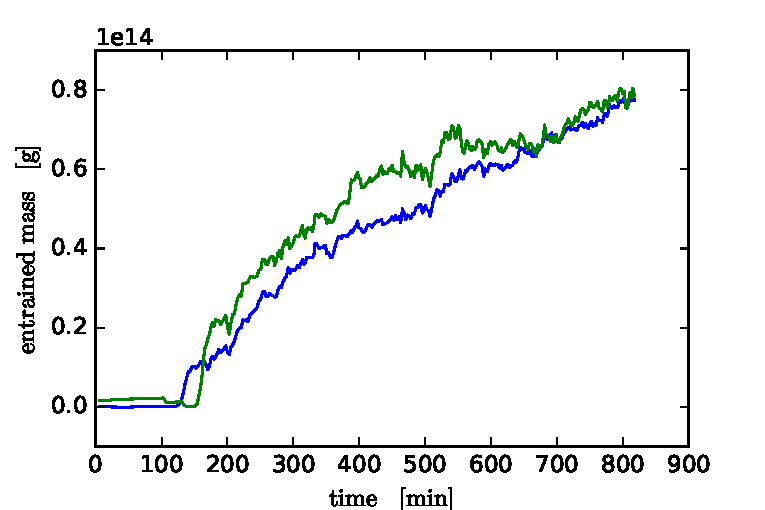
\includegraphics[width=0.5\textwidth]{./img/ent.pdf}\label{fig:ent}}
	\caption{Time evolution of the parameters needed to compute the bulk-Richardson number and of the entrained mass at the boundaries. Blue lines represent the upper boundary, green lines the lower boundary.}
	\label{fig:2dparam}
\end{figure}
We plot in Figure (\ref{fig:boundpos}) the boundaries positions over time. Shaded regions represent the boundary thickness (calculated as the boundary position standard deviation). Convection clearly starts at about $t=150 \mathrm{min}$. After a transition period of about $50 \mathrm{min}$ we can clearly see that there is a migration of the upper boundary upward and of the lower boundary downward, which is fairly stable over the run. Specifically in the upper case it starts in the middle of the simulated region and ends up at $\simeq 2.0 \times 10^{6} \ \mathrm{cm}$, for the lower case it starts at $\simeq - 3.1 \times 10^{6} \ \mathrm{cm}$ and moves downwards to $\simeq - 4.5 \times 10^{6} \ \mathrm{cm}$. The boundaries thickness is also overall stable. As previously mentioned an Eulerian study is impracticable for this phenomenon, because it is hard to quantify how much of the boundary migration in an Eulerian frame is due to the entrainment and how much due to the adiabatic expansion of the fluid. We observe a decrease in density in the central region of a few percent, and we presume the volume expands consequently. 

In Figure (\ref{fig:2dparam}) we plot the parameters relevant to our analysis. 
\begin{figure}[t!]
\centering
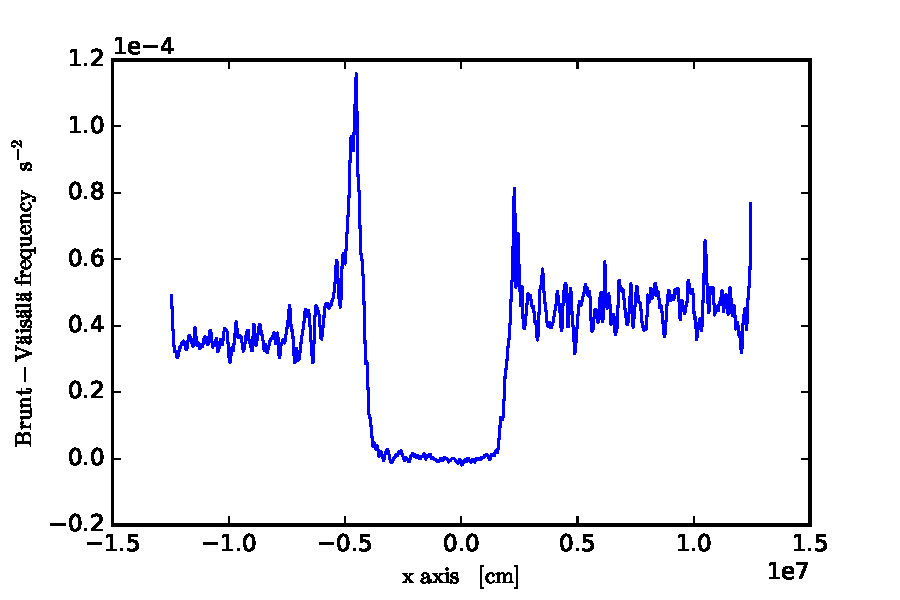
\includegraphics[width=0.6\textwidth]{./img/brunt}
\caption{Horizontal average of the Brunt-Väisälä frequency at about $t=500 \ \mathrm{min}$.}
\label{fig:brunt}
\end{figure}
The first ingredient of the bulk-Richardson number is the buoyancy jump $\Delta b$, that we plot in figure \ref{fig:delb}. In both cases there is an increasing trend, more significant in the lower boundary. This plot shows one of the biggest challenges of running simulations to study differentially the bulk-Richardson number: it is extremely hard to obtain a run where all the parameters ($\Delta b$, $L$, $\sigma_t$ and $M_{\mathrm{E}}$) are constant over time. Hence one finds itself in the inconvenient situation of having to average over values that span a full order of magnitude with a strong increasing or decreasing trend, and the quality of the analysis is consequentially affected by this uncertainty. 

\begin{figure}[t!]
\centering
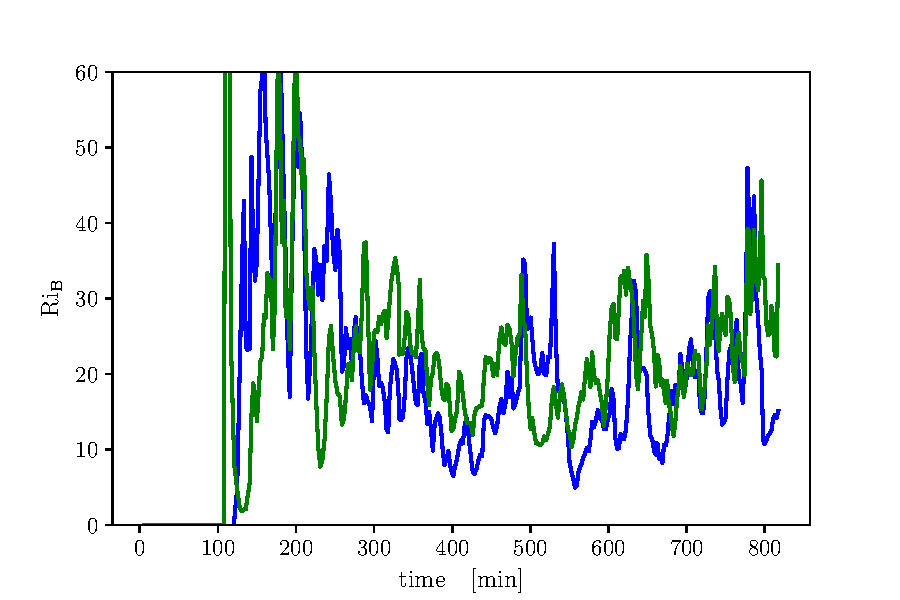
\includegraphics[width=0.6\textwidth]{./img/bulk.pdf}
\caption{Time evolution of the bulk-Richardson number. The blue line represents the upper boundary, the green line the lower one.}
\label{fig:bulk}
\centering
\end{figure}
Notice that the lower boundary is stiffer than the upper one (the buoyancy jump is higher, hence the bulk-Richardson number) even if in the initial setup the Brunt-Väisälä frequency is the same for the two stable regions. Recall that the Brunt-Väsälä frequency $N^2$ is the quantity we integrate in equation (\ref{eq:buoyancyjump}) over the boundary thickness in order to calculate $\Delta b$. Looking at Figure (\ref{fig:brunt}) it is clear that at the convective boundaries spikes arise during the simulation in the Brunt-Väisälä frequency, and in the lower case it is more pronounced. Obviously when integrated over the interface, this gives rise to a bigger buoyancy jump. These spikes in the Brunt-Väisälä frequency at the interfaces were also found by Arnett \emph{et al.} (2015).

In Figure (\ref{fig:len}) we plot the turbulent length scale $L$ over time. In this case we only calculated $L$ at the center of the convective layer, so this value will be used both for the upper and lower boundary analysis. The length scale at the interfaces has a value which is overall comparable, but it is affected by some spikes, reason for which we decided to calculate it in a fully convective region. The turbulent length scale is the parameter that takes more time to stabilize, becoming ultimately stable at around $t = 300 \mathrm{min}$. 
 
In Figure (\ref{fig:sigt}) we plot the turbulence absolute Mach number standard deviation at the convective interfaces over time. It is overall constant, with a slight trend to increase. This result has been obtained after extensive tests to correctly tune the heating function. It is in fact extremely hard to forecast the turbulence velocity by the heating generation and its time evolution. This problem perfectly shows the non-linearity of hydrodynamics as a theory.

In Figure (\ref{fig:ent}) the entrained mass over time. As already mentioned we will perform a Lagrangian study of entrainment, because it is impracticable to quantify how much of the boundary migration is due to the entrained mass or to the adiabatic expansion of the fluid. After an initial spike of entrained mass, we notice that also the entrainment rate stabilizes. We calculate the entrainment rate by fitting the entrained mass over time between $t = 300 \mathrm{min}$ until the end of the simulation, and by taking the angular coefficient of the resulting fit. 

We show in Figure (\ref{fig:bulk}) the bulk-Richardson number over time. Blue lines represent the upper boundary, green lines the lower boundary. At around $t=\mathrm{300 \ min}$, when the entrainment becomes linear and we start our analysis, the bulk-Richardson number still oscillates over half an order of magnitude. This obviously deeply affects our data analysis, making necessary a large amount of runs to collect as much data as possible. This also makes a differential study of the entrainment over time impracticable. 

For every 2D or 3D run we will extrapolate the relevant parameters and present them in the following layout
\begin{center}
 \begin{tabular}{l|c|c}
	 Run &2d0.7-0.01U&2d0.7-0.01L\\
	  	\hline
	   $\Delta b$ $(\mathrm{cm/s^{2}})$&$ 18.17 \pm 3.62 $&$27.68 \pm 7.18$\\
		\hline
	   $\sigma_t$ $(\mathrm{cm/s})$ &$ 1118 \pm 202 $&$1190 \pm 218$\\
		\hline
	   $L$ $(\mathrm{cm})$&$(10.88 \pm 2.56) \times 10^5$&$(10.88 \pm 2.56) \times 10^5$\\
		\hline
	   $Ri_{\mathrm{B}}$& $17.070 \pm 7.407 $&$21.622 \pm 6.538$\\
		\hline
	   $\dot{M}_{\mathrm{E}}$ $(\mathrm{g/s})$ &$(1.287 \pm 0.006) \times 10^9$&$(9.125 \pm 0.015) \times 10^8$\\
      \end{tabular}
 \end{center}
 Where the U at the end of the run name stands for upper boundary, and the L for lower boundary. 

 \new{

}
\subsection{Resolution study}
\begin{figure}[t!]
  \centering
  \subfloat[Mach number profile for the $2048 \times 1024$ run.]{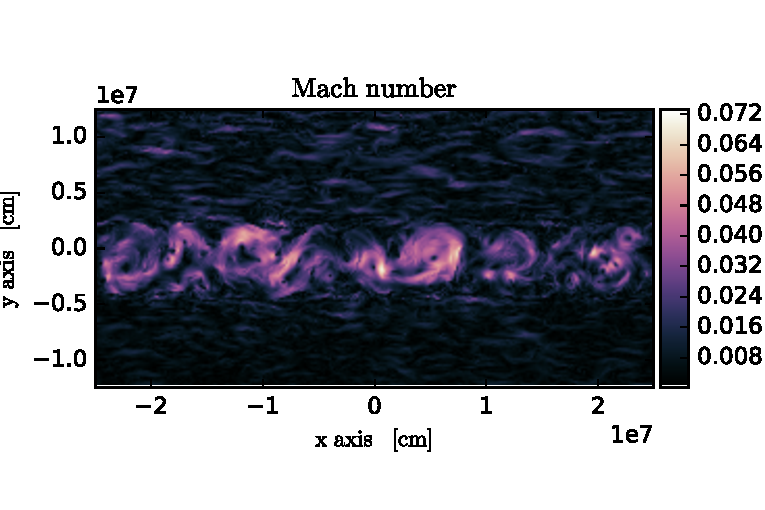
\includegraphics[width=12.cm]{./img/machhighres.pdf}}
  \centering
      \hfill
    \subfloat[Mach number profile for the $512 \times 256$ run.]{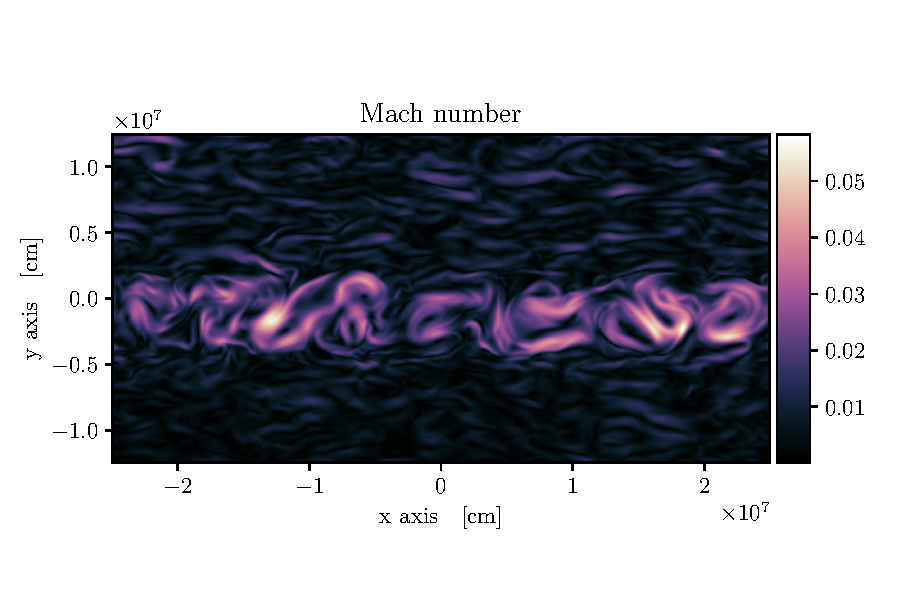
\includegraphics[width=12.cm]{./img/machlowres.pdf}}
    \caption{\new{Turbulent structures at different resolutions at about $t=500 \ \mathrm{min}$. Notice the higher Mach number in the $2048 \times 1024$ run due to lower numerical viscosity (see text).}}
    \label{fig:differentialmach}
 \end{figure}
In the last section we analyzed the run 2d0.10-0.80. What we will do in this section is to compare the previous results with the ones obtained by running the same setup on smaller resolutions, in order to understand if we are properly resolving the system. 

The same setup was run on a $1024 \times 512$ and $512 \times 256$. As expected, the highest resolution run shows smaller and more refined turbulent structures in the convective region, while in the smallest run we observe less eddies but of bigger size (see figure \ref{fig:differentialmach}).

We report in the following table the relevant parameters of the upper boundary for the different resolution runs.

\begin{center}
 \begin{tabular}{l|c|c|c}
	 Run &$2048 \times 1024$ U& $1024  \times 512$ U& $512 \times 256$ U\\
	  	\hline
		$\Delta b$ $(\mathrm{cm/s^{2}})$ & $ 18.17 \pm 7.41 $ & $15.48 \pm 2.31$ & $12.82 \pm 2.40$\\
		\hline
		$\sigma_t$ $(\mathrm{cm/s})$ & $ 1118 \pm 202 $ & $1020 \pm 196$ & $970 \pm 233$\\
		\hline
		$L$ $(\mathrm{cm})$&$(10.88 \pm 2.56) \times 10^5$ & $(11.07 \pm 3.30) \times 10^5$ & $(11.50 \pm 1.71) \times 10^5$\\
		\hline
		$Ri_{\mathrm{B}}$& $17.070 \pm 7.407 $ & $17.694 \pm 8.397 $ & $17.598 \pm 7.663$\\
		\hline
		$\dot{M}_{\mathrm{E}}$ $(\mathrm{g/s})$ &$(1.287 \pm 0.006) \times 10^9$&$(1.255 \pm 0.013) \times 10^9$ & $(1.174 \pm 0.016) \times 10^9$\\
      \end{tabular}
 \end{center}
 \new{
We observe that all the parameters are overall constant, within a $10 \%$ oscillation range. Woodward \textit{et al.} (2016) found that the entrainment rate decreases exponentially with the enhancement of the resolution, before converging to the physical value. In our case we observe a constant entrainment (with a slight increasing trend, we presume due to second order phenomena), hence we can safely assume that even in the lowest resolution case we are properly resolving the system. Notice that the turbulence standard deviation increases with the resolution as expected, because of the higher Reynolds number due to smaller numerical viscosity. 

One could still point out that the convergence reached in a 2D setup does not imply a convergence in 3D, but being that 3D simulations are computationally so expensive, it is impracticable for us to test this hypothesis.

Even at the lower boundary all the parameters oscillate within a $10 \%$ range. The only exception is the bulk-Richardson number but this is affected by a significant error in the lower resolution runs. Again in the higher resolution case the turbulence standard deviation is higher, as the entrainment rate.
\begin{table}\caption{ciao}
 \begin{tabular}{l|c|c|c}
	 Run &$2048 \times 1024$ L& $1024  \times 512$ L& $512 \times 256$ L\\
	  	\hline
		$\Delta b$ $(\mathrm{cm/s^{2}})$ & $ 27.62 \pm 6.54 $ & $25.85 \pm 6.48$ & $25.46 \pm 6.15$\\
		\hline
		$\sigma_t$ $(\mathrm{cm/s})$ & $ 1190 \pm 202 $ & $985 \pm 179$ & $977 \pm 143$\\
		\hline
		$L$ $(\mathrm{cm})$&$(10.88 \pm 2.56) \times 10^5$ & $(11.07 \pm 3.31) \times 10^5$ & $(11.50 \pm 1.71) \times 10^5$\\
		\hline
		$Ri_{\mathrm{B}}$& $21.622 \pm 6.538 $ & $31.934 \pm 17.718 $ & $33.334 \pm 17.721$\\
		\hline
		$\dot{M}_{\mathrm{E}}$ $(\mathrm{g/s})$ &$(9.252 \pm 0.015) \times 10^8$&$(1.006 \pm 0.017) \times 10^9$ & $(1.026 \pm 0.031) \times 10^9$\\
      \end{tabular}
\end{table}
}


\subsection{Differential 2D study}
\new{
	
}

\section{3D simulations}

\new{
	After having correctly tuned the heating function in a 2D setup, we switched to a 3D setup. Two simulations were run: 3d0.5-100 and 3d0.1-080, where the $0.5$ and $0.1$ stand again for the fraction $\nabla T / \nabla$ and the $100$ and $080$ stand for the percentage of the heating referring to the arbitrary value of $2.309 \times 10^{18} \mathrm{erg/s}$. These two values have been chosen in order to space as much as possible the resulting bulk-Richardson numbers, by generating a relatively stronger turbulence with a softer boundary (3d0.5-100) and a weaker turbulence with a stiffer boundary (3d0.1-080). As in the 2D case, the heating function has a Gaussian profile peaked in the convective zone and decreasing in time.

	Both runs were performed on a $512 \times 256 \times 512$ uniform Cartesian grid. The first simulation was run locally on the IWR cluster in Heidelberg and scaled over $512$ haswell cores, for a total run time of about 2 weeks. The second was run on the JUQUEEN machine at JSC and scaled over an entire rack ($16384$ cores) for four days. Although SLH scales very well even on tens of thousands of cores, on JUQUEEN a higher number of CPU hours was needed for two reasons. First of all the PowerPC\textregistered \ A2 processors (IBM) of JUQUEEN are optimized to obtain the highest efficiency in terms of computations per watt, rather that per core. Second the PowerPC\textregistered \ A2 belongs to a earlier architecture generation than the haswell (Intel) one.

}

\subsection{Evolution of a 3D run}
\new{
We analyze the run 3d0.1-080.

Similarly to the 2D case, convection start at $t \simeq 250 \mathrm{min}$ and in figure \ref{fig:3dsingle} is visible the growth of the convective region by entrainment of stable medium.

In comparison to the 2D case we add more heating into the fluid and we simulate a stiffer boundary (that should help contain the entropy raise better than a softer one), nevertheless the turbulence Mach number is lower. This result was expected because, as previously mentioned, three-dimensional turbulence has a different behavior compared to the two-dimensional one. In our case the 3D turbulence standard deviation was always a factor of a few lower than in the 2D case, which is in agreement with what found by Meakin and Arnett (2007) in their core-convection simulation. 
\begin{figure}[t!]
      \centering
        \subfloat[Mach number profile over time.]{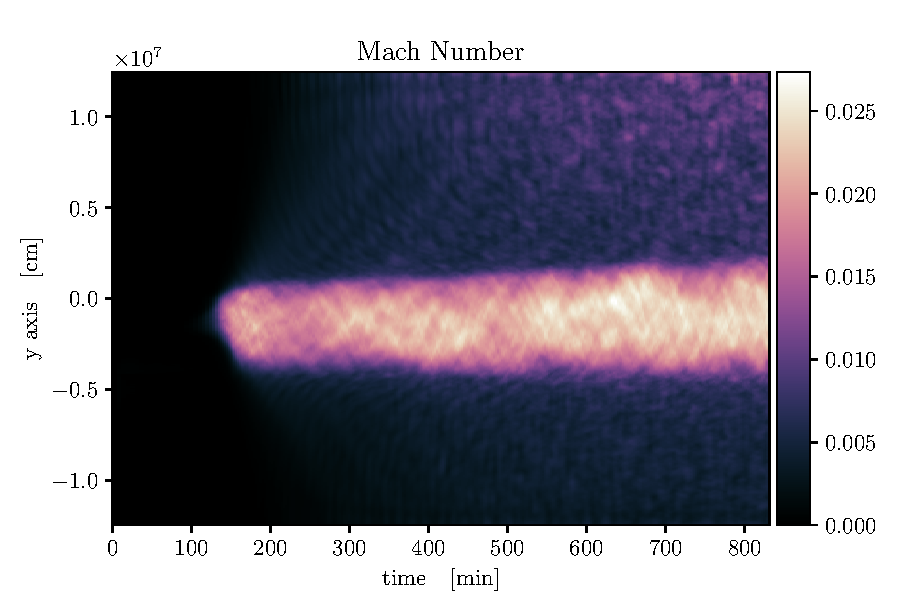
\includegraphics[width=10cm]{./img/mach.pdf}\label{fig:mach3d}}
     \centering
	\hfill
        \subfloat[Entrainment of passive scalar from the upper stable region into the convective region.]{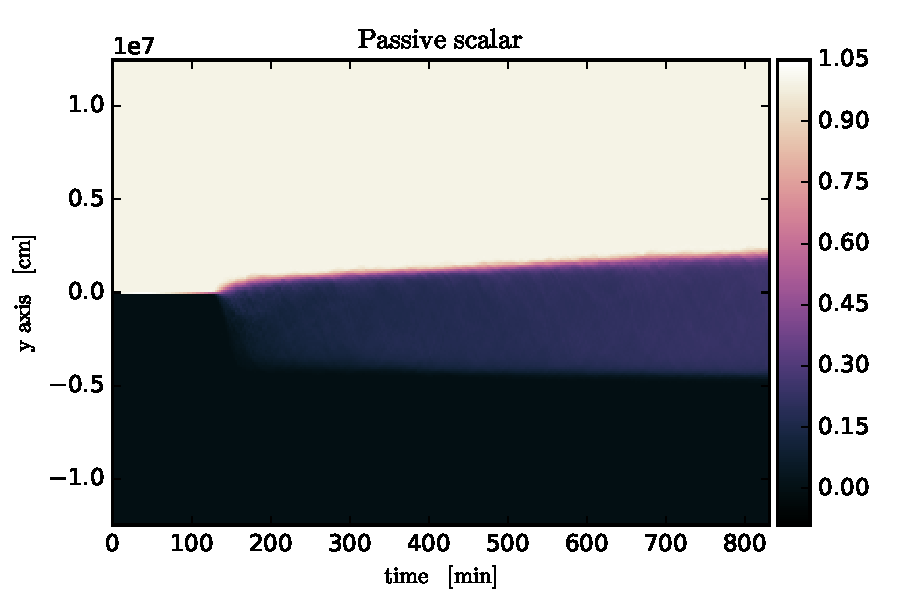
\includegraphics[width=10cm]{./img/ps2.pdf}\label{fig:ps3d}}
	\caption{Time evolution of a 3D run. In comparison to the 2D case less output files were saved, hence the lower resolution in time.}
	\label{3dsingle}
\end{figure}
The different turbulence configuration between the 2D and 3D case can be better understood by comparing figure \ref{} with figure \ref{mach3d}. In the previous section we showed that, the better the resolution, the more refined and complex the turbulent structure. When running a 3D simulation, even by looking at a $512 \times 256$ section of the grid, the Mach number already shows a very sophisticated and convoluted shape, comparable to the $2048 \times 1024$ 2D case.
}
\subsection{Differential 3D study}
